\subsection{Electricity and Water Usage Correlation}
%From the above electricity and water disaggregation, 
%we observe that some devices, such as washing machine, use both electricity and water. 
%We extend our multivariate episode mining approach 
%from disaggregating two time series of hot water and cold water, 
%to three time series of hot water, cold water and electricity. 

We discover that water usage is more like a series of human behavior, as in Figure \ref{fig_bathroomBehavior}.
One person turns on the light L007 in the bathroom,  uses the toilet, flushes and wash hands,
accompanied by  taking  a shower and leaving the bathroom with the light turned off. 
\begin{figure}[!t]
\centering
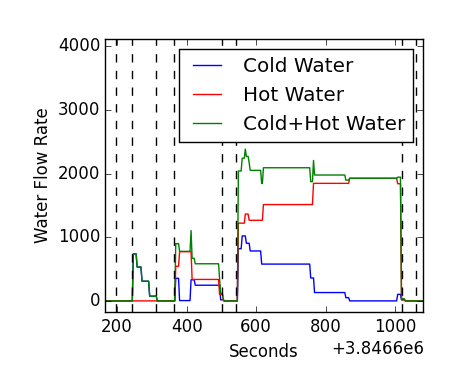
\includegraphics[width=0.7\textwidth]{multidisaggfig/bathroomBehavior.png}
\caption{Human behavior in bathroom by using down toilet, down sink and shower. The dashed lines denote 
a series of events: light L007 on, down toilet on,  down toilet off, down sink on, down sink off, shower on, shower off, light L007 off. }
\label{fig_bathroomBehavior}
\end{figure}

\begin{comment}
\begin{table}[!t]
\renewcommand{\arraystretch}{1.3}
\caption{Washing Machine Disaggregation with Multivariate Episode Mining}
\label{table_washingMachineDisagg}
\centering
\begin{tabular}{|c|c|c|c|c|}
\hline
Aggregated Data & Disaggregation Type& Precision  & Recall & F-Measure\\
\hline
\hline
Electricity & Single & 0.8 & 0.9 & 0.88\\
\hline
Water & Multivariate& 0.8 & 0.9 & 0.88\\
\hline
Electricity and Water & Multivariate & 0.8 & 0.9 & 0.88\\
\hline
\end{tabular}
\end{table}
\end{comment}